
\chapter{Introduction}
    Workflow Management Systems are systems designed to facilitate and manage
    tasks within an organisation. These tasks are topologically organised and
    the system then executes the workflow
    such that each task's dependencies are first met. Such a system would allow a user to
    set up, monitor and execute tasks \cite{slot2005workflow}.

    Workflow systems have been successfully implemented in various
    business and Scientific fields \cite{Brahe:2007:SWW:1316624.1316661}.
    This has not only increased productivity but in the field of
    science has allowed that the reproducibility of results be greatly
    increased\cite{4721191}.

    In recent years scientific discovery has move towards being more data-driven\cite{gray2007escience}.
    This has created a process where large amounts of data is collected, processed
    and then analysed to produce results. Where in the past results were based in simulating
    and evaluating experimental models, it has become important that results are based in
    data. This method has been highly effective across various fields including: Pharmacology\cite{harpaz2012novel},
    Astrophysics\cite{thomas2011synapps} and Bioinformatics\cite{greene2010integrative}.
    In order to support these processes, sophisticated tools are required to process
    and analyse this data\cite{shneiderman2002inventing}.

    Management of this data is an extremely important process that ensures the
    ability to produce these scientific results\cite{gray2005scientific}. Workflow
    Management Systems, is an important component in this as it provides a means
    to very accurately record the scientific process followed  \cite{davidson2007provenance}.
    Effective management of the data allows for complex analysis to be performed,
    which ultimately leads to scientific discovery\cite{ludascher2009scientific}.




\section{Zamani Project and Cultural Heritage}
    The \emph{Zamani Project},\footnote{Zamani Project:http://www.zamani-project.org/}
    based at the Geomatics Department at the University of Cape Town,
    aims to accurately record the physical and architectural nature
    and dimensions of African Heritage sites.

    Heritage sites are mapped using sophisticated technology that is
    used to create a variety of digital objects, such as:
    \begin{inparaenum}[i)] \item Geographic Information Systems; \item 3D
    Computer Models; and \item Panoramic Photographs\end{inparaenum}.
    The team has recorded sites in Ghana, Mali, Kenya, Ethiopia, Tanzania and
    South Africa. Other sites are currently in progress or being planned.

    These are some of the best, and most accurate heritage documentation
    in the world.
    A very large collection of data items has to be managed
    within the project. Currently, the team is experiencing difficulty managing
    the vast amount of data items that needs to be processed. The size of these
    data items provides a challenge to traditional workflow systems that are
    currently available.

    To document these heritage sites require a great deal of effort. The process includes
    the capture, storage, manipulation, analysis and management of this geographic,
    architectural and photographic data. This data is very large and diverse. It gets
    used in very diverse ways. This involves processes abstracting these data
    items into various forms. Managing the data in such a way that it is accessible
    at any point presents a challenge due to the size of the data.

    Currently, the documentation process of the heritage sites involves the data being
    manually copied to each point where it is required. This is an extremely slow and
    laborious process. By automating this process time could be saved.



\section{General Outline}
    The project is divided into two major components. The first is a
    workflow management system developed by Michiel Johan Baird. The
    second is an indexing and streaming system for large point clouds
    developed by Timothy Trewartha. These two components aim to solve some
    of the challenges faced by the members of the Zamani Project.
    \subsection{Workflow Managment System}
        In order to assists with the difficulty in managing the data and the tasks involved
        in creating the heritage data, a Workflow Management System was developed using
        the requirements of the team.

        This system is able to handle both automated and manual user tasks. The
        aim is to increase the efficiency of the task execution and improving
        reusability between different heritage sites sites.

    \subsection{Point Cloud Indexing}
        The other component tackles the difficulty involved in managing large
        point clouds. The approach taken is to build an index for the point cloud. This index
        allows for efficient region extraction. It also allows the user to specify the resolution at which
        they wish the extraction to be performed.
        The system also enables the extractions from the point cloud index to
        be streamed from a central server. For example, using the index a low resolution
        representation can be efficiently extracted and sent to the client. Alternatively, the user may request
        a high resolution extraction of a subregion.
\\

    \noindent These two separate components can interact in a number of ways. For
        example, at various
        stages the Workflow Management System requires point clouds as input
        to certain processes.
        This input can be efficiently extracted from the indexed point cloud
        using the point cloud
        streaming system. Alternatively, if the Workflow Managment System
        produces a point cloud
        as output (after cleaning for example) it can be sent to the indexer
        so it can be more efficiently
        accessed further down the workflow pipeline. System.

    This report discusses the development and evaluation of the Workflow Management System.

\section{Problem Statement}

    Workflow management systems decompose complicated procedures into small atomic tasks
    that are dependent on one an other\cite{Taylor:2006:WES:1196459}. This decomposition
    often leads to an increase in overall efficiency of the process. Workflow Systems
    are particularly efficient in instances where there are multi-person teams and work
    is done in mostly independent tasks. These are the exact conditions that
    are present within the Zamani-project.

    The aim of this project is to develop and evaluate a system that is is applicable
    to workflows similar to those found within the Zamani Project. This should allow the
    system to: \begin{inparaenum}[i)] \item interface with existing systems; \item manage the
    work both at a site and a user level; \item provide local data availability when users
    require it for a task; and \item increase the overall efficiency of the process.
    \end{inparaenum}

\section{System Outline}
    This project is about a Workflow Management system that could effectively
    automate the management of the heritage preservation processes.
	This would manage the process starting from the raw scans and photographs
	through the creation of all the digital artifacts. Figure~\ref{intro:basic}
	shows the simplified operation of the system.
	\begin{figure}[!h]
		\begin{center}
			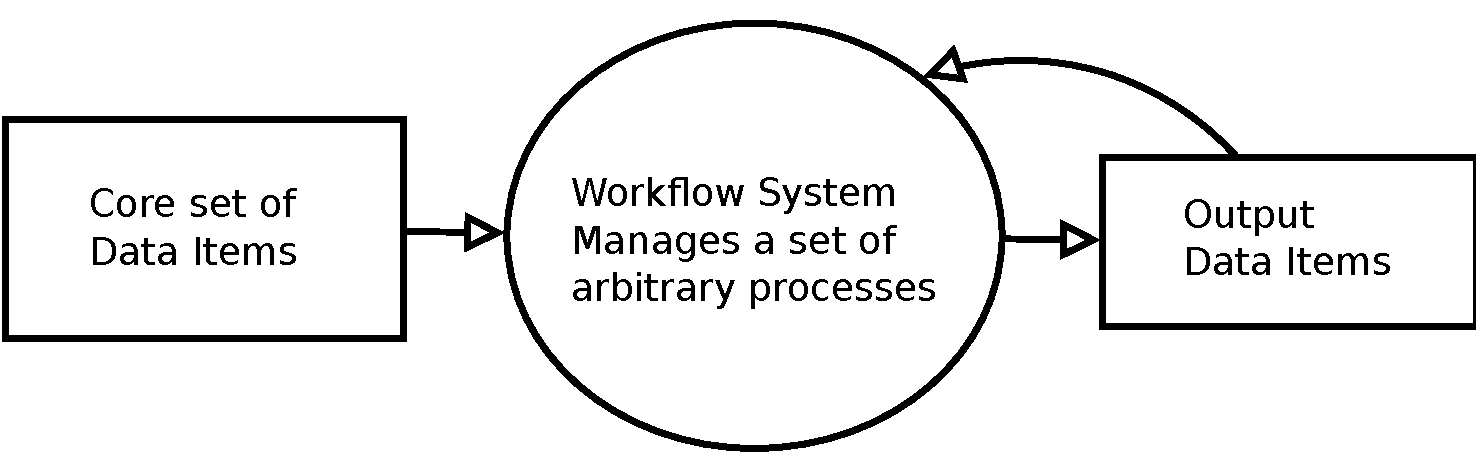
\includegraphics[scale=0.34]{figures/basic_system.pdf}
		\end{center}
		\caption{Basic System Overview}
		\label{intro:basic}
	\end{figure}

	\noindent The system would starts with a
	core set of input files. The workflow is then executed, which initiates a set
	of topologically-sorted tasks. These tasks would then be executed in order, such that
    the processes then generate the full set of output data items. These output items can then
    be used as input files in remaining tasks.

    These processes can be ordered into two main categories:
    \begin{inparaenum}[(i)]
        \item tasks that can automatically be executed by the system; and
        \item tasks that need to be completed by a user.
    \end{inparaenum} The system aims to coordinate an automate these tasks to
    the maximum extent possible whilst managing the information.

    Executing these processes involves using various software packages.
    This functionality can not be replaced by the system so it would need
    to be integrated in a very general way, this would be done by using wrapper
    software software that would use these applications to complete the required goal.

\section{System Evaluation}
    In order to determine the applicability of the proposed solution, the system
    was evaluated in the following ways:

    \begin{description}
        \item[Partial Integration Case Study]\hfill \\
            In order to determine whether the proposed system
            would be applicable to the problem at hand, a portion of the workflow
            of an existing site was implemented and tested within the system. This
            test provides a means to determine whether the problem could be solved
            by the proposed system.
        \item[User Experience Testing] \hfill \\
            Even the most effective system can fail if it cannot
            be successfully be adopted by users. Therefore, the system's
            user experience was tested. This allowed problems to be detected and
            shortcomings of the system to be identified\cite{tullis2008measuring}.
    \end{description}

\section{Legal and Ethical Issues}
    All the software used in the development of the workflow system
    is either free or open source. If this project were to continue
    or be extended, there would not be any legal issues. The core
    of the system is written using the Django Framework, using Python.
    These are, respectively, licenced by the Django Licence and the PSF
    license. Further tools used during the implementation include Javascript
    which is licenced under the LGPL.
    JQuery, JsPlumb and tablesorter, which are dual licenced the  MIT license
    and GPL, Version 2.

    Further data and information was obtained from the Zamani Project for
    testing the application. Permission was obtained to use this data.

    User testing was also done during the course of the project. For
    this purpose, ethical clearance was granted from the Faculty of
    Science Research Ethics Committee. Access to UCT Students was also
    granted by the Department of Student Affairs.

\section{Report Outline}
    This report outlines the design, implementation and evaluation
    of \emph{Zamani Workflow}, a workflow system that sets out to
    solve the data management problems experienced within the
    Zamani Project. The report starts with a review of the literature in
    Chapter~\ref{chap1}.

    This is then followed by the Design and Implementation of the system
    in Chapter~\ref{chap2}. The considerations for the design are defined
    before the full system design is reported. This design process involved
    three iterations.

    The final system in then evaluated in Chapter~\ref{chap3}. This was accomplished
    using a \emph{User Experience} evaluation and an \emph{Integration Case Study}.

    The report is then concluded in Chapter~\ref{chap4} where the system is
    reviewed. Here possible future avenues of research is discussed that could
    be used to build on the project.
